\begin{figure*}[!]
  \centering
  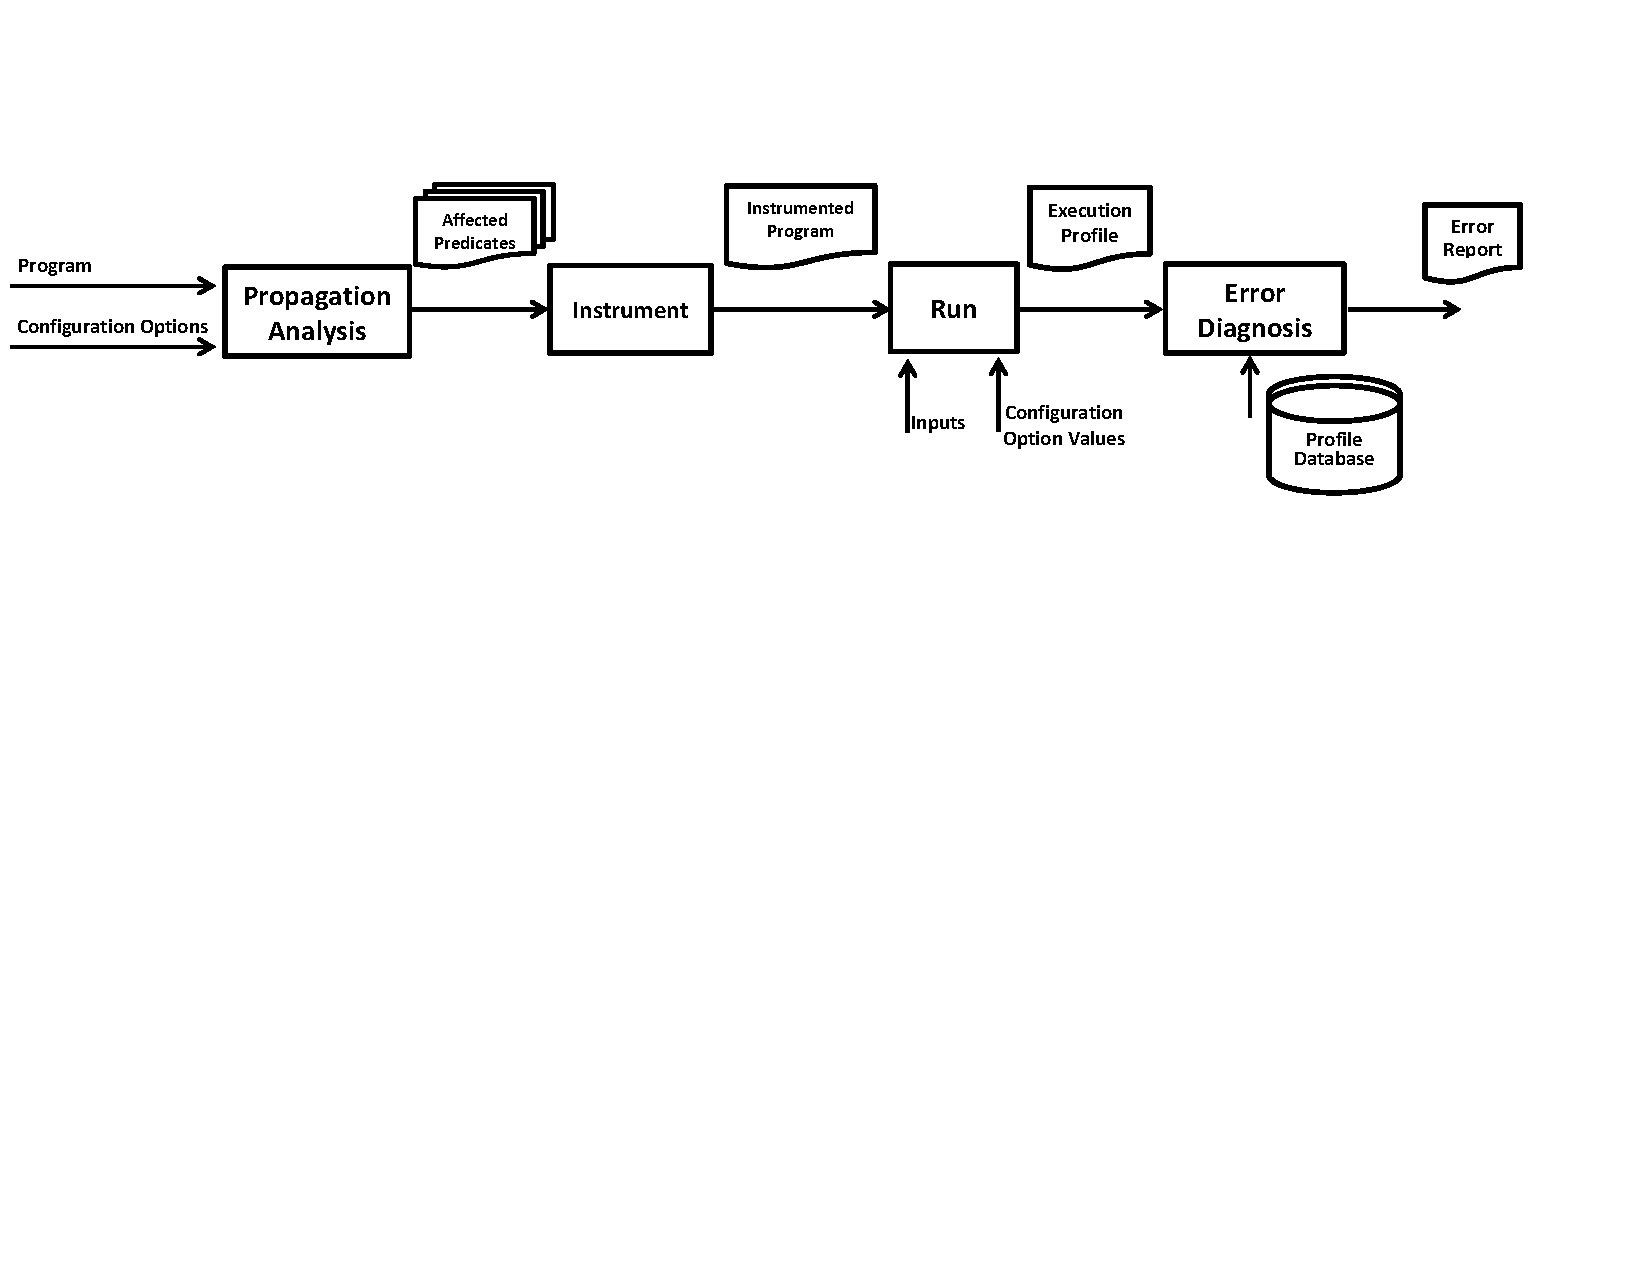
\includegraphics[scale=0.600]{architecture}
  \vspace*{-2.0ex}\caption {{\label{fig:workflow} The workflow of our configuration error diagnosis technique.
``Propagation Analysis'' is described in Section~\ref{sec:prop}.
The ``Instrument'' and ``Run'' components correspond to the Configuration Behavior Profiling step in Section~\ref{sec:profiling}.
``Deviation Analysis'' is described in Section~\ref{sec:analysis}.
}}
%\todo{The paper sometimes uses the terminology ``execution profile'' and
%  sometimes ``trace''.  Please be consistent.  I like ``execution profile''
%  better, because there is no temporal information about ordering in it.}
%\todo{The use of ``inputs'', in this figure and elsewhere, suggests that
%  the user runs multiple executions.  In fact, it is one execution, right?
%  I would change the arrow label ``inputs'' to ``input'' and
%  ``configurations'' to ``configuration''.  I would also label them as
%  ``bad runs''.  Then, I would change the database symbol's label from
%  ``Profile Database'' to ``Profile Database (good runs)''.}
\end{figure*}

\label{dummy-for-etags-workflow}
